\documentclass{article}
\usepackage[english]{babel}
\usepackage{geometry,amsmath,graphicx,hyperref,alltt,theorem}
\geometry{letterpaper}

%%%%%%%%%% Start TeXmacs macros
\catcode`\<=\active \def<{
\fontencoding{T1}\selectfont\symbol{60}\fontencoding{\encodingdefault}}
\catcode`\>=\active \def>{
\fontencoding{T1}\selectfont\symbol{62}\fontencoding{\encodingdefault}}
\newcommand{\tmem}[1]{{\em #1\/}}
\newcommand{\tmstrong}[1]{\textbf{#1}}
\newcommand{\tmverbatim}[1]{\text{{\ttfamily{#1}}}}
\newenvironment{tmcode}[1][]{\begin{alltt} }{\end{alltt}}
{\theorembodyfont{\rmfamily\small}\newtheorem{exercise}{Exercise}}
%%%%%%%%%% End TeXmacs macros

\begin{document}

{\class{Functional Programming}}

{\title{Streams and lazy evaluation}}

\begin{exercise}
  My first impulse was to define lazy list functions as here:
  
  \\
  {\hlkwa{let rec }}{\hlstd{wrong\_lzip }}{\hlopt{=
  }}{\hlkwa{function}}{\hlendline{}}\\
  {\hlstd{ {\hlopt{\textbar}} }}{\hlkwd{LNil}}{\hlopt{, }}{\hlkwd{LNil
  }}{\hlopt{-> }}{\hlkwd{LNil}}{\hlendline{}}\\
  {\hlstd{ {\hlopt{\textbar}} }}{\hlkwd{LCons
  }}{\hlopt{(}}{\hlstd{a1}}{\hlopt{, }}{\hlkwa{lazy }}{\hlstd{l1}}{\hlopt{),
  }}{\hlkwd{LCons }}{\hlopt{(}}{\hlstd{a2}}{\hlopt{, }}{\hlkwa{lazy
  }}{\hlstd{l2}}{\hlopt{) ->}}{\hlendline{}}\\
  {\hlstd{ \ \ \ \ }}{\hlkwd{LCons }}{\hlopt{((}}{\hlstd{a1}}{\hlopt{,
  }}{\hlstd{a2}}{\hlopt{), }}{\hlkwa{lazy }}{\hlopt{(}}{\hlstd{wrong\_lzip
  }}{\hlopt{(}}{\hlstd{l1}}{\hlopt{,
  }}{\hlstd{l2}}{\hlopt{)))}}{\hlendline{}}\\
  {\hlstd{ {\hlopt{\textbar}} {\textunderscore} }}{\hlopt{-> }}{\hlstd{raise
  }}{\hlopt{(}}{\hlkwd{Invalid{\textunderscore}argument
  }}{\hlstr{"lzip"}}{\hlopt{)}}{\hlendline{}}\\
  {\hlendline{}}\\
  {\hlkwa{let rec }}{\hlstd{wrong\_lmap f }}{\hlopt{=
  }}{\hlkwa{function}}{\hlendline{}}\\
  {\hlstd{ {\hlopt{\textbar}} }}{\hlkwd{LNil }}{\hlopt{->
  }}{\hlkwd{LNil}}{\hlendline{}}\\
  {\hlstd{ {\hlopt{\textbar}} }}{\hlkwd{LCons
  }}{\hlopt{(}}{\hlstd{a}}{\hlopt{, }}{\hlkwa{lazy }}{\hlstd{l}}{\hlopt{) ->
  }}{\hlkwd{LCons }}{\hlopt{(}}{\hlstd{f a}}{\hlopt{, }}{\hlkwa{lazy
  }}{\hlopt{(}}{\hlstd{wrong\_lmap f l}}{\hlopt{))}}{\hlendline{}}\\
  
  
  What is wrong with these definitions -- for which edge cases they do not
  work as intended?
\end{exercise}

\begin{exercise}
  Cyclic lazy lists:
  \begin{enumerate}
    \item Implement a function \tmverbatim{cycle : 'a list -> 'a llist} that
    creates a lazy list with elements from standard list, and the whole list
    as the tail after the last element from the input list.
    
    \tmverbatim{[a1; a2; ...;
    aN]}$\mapsto$\raisebox{-0.415018574208385\height}{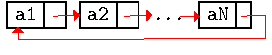
\includegraphics[width=4.57183851502033cm,height=0.926964449691722cm]{lecture07-exercises-via-latex-1.pdf}}
    
    Your{\tmstrong{}} function \tmverbatim{cycle} can either return
    \tmverbatim{LNil} or fail for an empty list as argument.
    
    \item Note that \tmverbatim{inv\_fact} from the lecture defines the power
    series for the $\exp (\cdot)$ function ($\exp (x) = e^x$). Using
    \tmverbatim{cycle} and \tmverbatim{inv\_fact}, define the power series for
    $\sin (\cdot)$ and $\cos (\cdot)$, and draw their graphs using helper
    functions from the lecture script \tmverbatim{Lec7.ml}.
  \end{enumerate}
\end{exercise}

\begin{exercise}
  * Modify one of the puzzle solving programs (either from the previous
  lecture or from your previous homework) to work with lazy lists. Implement
  the necessary higher-order lazy list functions. Check that indeed displaying
  only the first solution when there are multiple solutions in the result
  takes shorter than computing solutions by the original program.
\end{exercise}

\begin{exercise}
  {\tmem{Hamming's problem}}. Generate in increasing order the numbers of the
  form $2^{a_1} 3^{a_2} 5^{a_3} \ldots p_k^{a_k}$, that is numbers not
  divisible by prime numbers greater than the $k$th prime number.
  \begin{itemize}
    \item In the original Hamming's problem posed by Dijkstra, $k = 3$, which
    is related to
    \href{http://en.wikipedia.org/wiki/Regular_number}{http://en.wikipedia.org/wiki/Regular\_number}.
  \end{itemize}
  Starter code is available in the middle of the lecture script
  \tmverbatim{Lec7.ml}:\\
  {\hlkwa{let rec }}{\hlstd{lfilter f }}{\hlopt{=
  }}{\hlkwa{function}}{\hlendline{}}\\
  {\hlstd{ {\hlopt{\textbar}} }}{\hlkwd{LNil }}{\hlopt{->
  }}{\hlkwd{LNil}}{\hlendline{}}\\
  {\hlstd{ {\hlopt{\textbar}} }}{\hlkwd{LCons
  }}{\hlopt{(}}{\hlstd{n}}{\hlopt{, }}{\hlstd{ll}}{\hlopt{)
  ->}}{\hlendline{}}\\
  {\hlstd{ \ \ \ \ }}{\hlkwa{if }}{\hlstd{f n }}{\hlkwa{then }}{\hlkwd{LCons
  }}{\hlopt{(}}{\hlstd{n}}{\hlopt{, }}{\hlkwa{lazy
  }}{\hlopt{(}}{\hlstd{lfilter f
  }}{\hlopt{(}}{\hlkwc{Lazy}}{\hlopt{.}}{\hlstd{force
  ll}}{\hlopt{)))}}{\hlendline{}}\\
  {\hlstd{ \ \ \ \ }}{\hlkwa{else }}{\hlstd{lfilter f
  }}{\hlopt{(}}{\hlkwc{Lazy}}{\hlopt{.}}{\hlstd{force
  ll}}{\hlopt{)}}{\hlendline{}}\\
  {\hlendline{}}\\
  {\hlkwa{let }}{\hlstd{primes }}{\hlopt{=}}{\hlendline{}}\\
  {\hlstd{ }}{\hlkwa{let rec }}{\hlstd{sieve }}{\hlopt{=
  }}{\hlkwa{function}}{\hlendline{}}\\
  {\hlstd{ \ \ \ \
  }}{\hlkwd{LCons}}{\hlopt{(}}{\hlstd{p}}{\hlopt{,}}{\hlstd{nf}}{\hlopt{) ->
  }}{\hlkwd{LCons}}{\hlopt{(}}{\hlstd{p}}{\hlopt{, }}{\hlkwa{lazy
  }}{\hlopt{(}}{\hlstd{sieve }}{\hlopt{(}}{\hlstd{sift p
  }}{\hlopt{(}}{\hlkwc{Lazy}}{\hlopt{.}}{\hlstd{force
  nf}}{\hlopt{))))}}{\hlendline{}}\\
  {\hlstd{ \ \ }}{\hlopt{\textbar }}{\hlkwd{LNil }}{\hlopt{->
  }}{\hlstd{failwith }}{\hlstr{"Impossible! Internal
  error."}}{\hlstd{{\hlendline{}}\\
  }}{\hlkwa{and }}{\hlstd{sift p }}{\hlopt{= }}{\hlstd{lfilter
  }}{\hlopt{(}}{\hlkwa{function }}{\hlstd{n }}{\hlopt{-> }}{\hlstd{n
  }}{\hlkwa{mod }}{\hlstd{p }}{\hlopt{<>
  }}{\hlnum{0}}{\hlopt{)}}{\hlendline{}}\\
  {\hlkwa{in }}{\hlstd{sieve }}{\hlopt{(}}{\hlstd{lfrom
  }}{\hlnum{2}}{\hlopt{)}}{\hlendline{}}\\
  {\hlendline{}}\\
  {\hlkwa{let }}{\hlstd{times ll n }}{\hlopt{= }}{\hlstd{lmap
  }}{\hlopt{(}}{\hlkwa{fun }}{\hlstd{i }}{\hlopt{-> }}{\hlstd{i }}{\hlopt{*
  }}{\hlstd{n}}{\hlopt{) }}{\hlstd{ll}}{\hlopt{;;}}{\hlendline{}}\\
  {\hlendline{}}\\
  {\hlkwa{let rec }}{\hlstd{merge xs ys }}{\hlopt{= }}{\hlkwa{match
  }}{\hlstd{xs}}{\hlopt{, }}{\hlstd{ys }}{\hlkwa{with}}{\hlendline{}}\\
  {\hlstd{ \ }}{\hlopt{\textbar }}{\hlkwd{LCons
  }}{\hlopt{(}}{\hlstd{x}}{\hlopt{, }}{\hlkwa{lazy }}{\hlstd{xr}}{\hlopt{),
  }}{\hlkwd{LCons }}{\hlopt{(}}{\hlstd{y}}{\hlopt{, }}{\hlkwa{lazy
  }}{\hlstd{yr}}{\hlopt{) ->}}{\hlendline{}}\\
  {\hlstd{ \ \ \ \ }}{\hlkwa{if }}{\hlstd{x }}{\hlopt{< }}{\hlstd{y
  }}{\hlkwa{then }}{\hlkwd{LCons }}{\hlopt{(}}{\hlstd{x}}{\hlopt{,
  }}{\hlkwa{lazy }}{\hlopt{(}}{\hlstd{merge xr
  ys}}{\hlopt{))}}{\hlendline{}}\\
  {\hlstd{ \ \ \ \ }}{\hlkwa{else if }}{\hlstd{x }}{\hlopt{> }}{\hlstd{y
  }}{\hlkwa{then }}{\hlkwd{LCons }}{\hlopt{(}}{\hlstd{y}}{\hlopt{,
  }}{\hlkwa{lazy }}{\hlopt{(}}{\hlstd{merge xs
  yr}}{\hlopt{))}}{\hlendline{}}\\
  {\hlstd{ \ \ \ \ }}{\hlkwa{else }}{\hlkwd{LCons
  }}{\hlopt{(}}{\hlstd{x}}{\hlopt{, }}{\hlkwa{lazy }}{\hlopt{(}}{\hlstd{merge
  xr yr}}{\hlopt{))}}{\hlendline{}}\\
  {\hlstd{ {\hlopt{\textbar}} r}}{\hlopt{, }}{\hlkwd{LNil }}{\hlopt{\textbar
  }}{\hlkwd{LNil}}{\hlopt{, }}{\hlstd{r }}{\hlopt{->
  }}{\hlstd{r}}{\hlendline{}}\\
  {\hlendline{}}\\
  {\hlkwa{let }}{\hlstd{hamming k }}{\hlopt{=}}{\hlendline{}}\\
  {\hlstd{ }}{\hlkwa{let }}{\hlstd{pr }}{\hlopt{= }}{\hlstd{ltake k primes
  }}{\hlkwa{in}}{\hlendline{}}\\
  {\hlstd{ }}{\hlkwa{let rec }}{\hlstd{h }}{\hlopt{= }}{\hlkwd{LCons
  }}{\hlopt{(}}{\hlnum{1}}{\hlopt{, }}{\hlkwa{lazy
  }}{\hlopt{(}}{\hlendline{}}\\
  {\hlstd{ \ \ }}{\hlopt{<}}{\hlkwd{TODO}}{\hlopt{> ))
  }}{\hlkwa{in}}{\hlendline{}}\\
  {\hlstd{ h}}{\hlendline{}}
\end{exercise}

\begin{exercise}
  Modify \tmverbatim{format} and/or \tmverbatim{breaks} to use just a single
  number instead of a stack of booleans to keep track of what groups should be
  inlined.
\end{exercise}

\begin{exercise}
  Add {\tmstrong{indentation}} to the pretty-printer for groups: if a group
  does not fit in a single line, its consecutive lines are indented by a given
  amount \tmverbatim{tab} of spaces deeper than its parent group lines would
  be. For comparison, let's do several implementations.
  \begin{enumerate}
    \item Modify the straightforward implementation of \tmverbatim{pretty}.
    
    \item Modify the first pipe-based implementation of \tmverbatim{pretty} by
    modifying the \tmverbatim{format} function.
    
    \item Modify the second pipe-based implementation of \tmverbatim{pretty}
    by modifying the \tmverbatim{breaks} function. Recover the positions of
    elements -- the number of characters from the beginning of the document --
    by keeping track of the growing offset.
    
    \item * Modify a pipe-based implementation to provide a different style of
    indentation: indent the first line of a group, when the group starts on a
    new line, at the same level as the consecutive lines (rather than at the
    parent level of indentation). 
  \end{enumerate}
\end{exercise}

\begin{exercise}
  Write a pipe that takes document elements annotated with linear position,
  and produces document elements annotated with (line, column) coordinates.
  
  Write another pipe that takes so annotated elements and adds a line number
  indicator in front of each line. Do not update the column coordinate. Test
  the pipes by plugging them before the \tmverbatim{emit} pipe.
  \begin{tmcode}
  1: first line
2: second line, etc.
  \end{tmcode}
\end{exercise}

\begin{exercise}
  Write a pipe that consumes document elements \tmverbatim{doc\_e} and yields
  the toplevel subdocuments \tmverbatim{doc} which would generate the
  corresponding elements.
  
  You can modify the definition of documents to allow annotations, so that the
  element annotations are preserved (\tmverbatim{gen} should ignore
  annotations to keep things simple):\\
  {\hlkwa{type }}{\hlstd{'a doc }}{\hlopt{=}}{\hlendline{}}\\
  {\hlstd{ \ }}{\hlkwd{Text }}{\hlkwa{of }}{\hlstd{'a }}{\hlopt{*
  }}{\hlkwb{string }}{\hlopt{\textbar }}{\hlkwd{Line }}{\hlkwa{of }}{\hlstd{'a
  {\hlopt{\textbar}} }}{\hlkwd{Cat }}{\hlkwa{of }}{\hlstd{doc }}{\hlopt{*
  }}{\hlstd{doc {\hlopt{\textbar}} }}{\hlkwd{Group }}{\hlkwa{of }}{\hlstd{'a
  }}{\hlopt{* }}{\hlstd{doc}}{\hlendline{}}
\end{exercise}

\begin{exercise}
  * Design and implement a way to duplicate arrows outgoing from a pipe-box,
  that would memoize the stream, i.e. not recompute everything ``upstream''
  for the composition of pipes. Such duplicated arrows would behave nicely
  with pipes reading from files.
  
  \raisebox{-0.459422933982026\height}{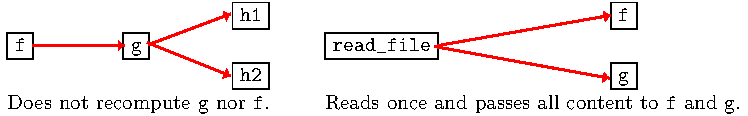
\includegraphics[width=12.5656401679129cm,height=1.9413616686344cm]{lecture07-exercises-via-latex-2.pdf}}
\end{exercise}

\end{document}
